Multicore architectures are changing the way we write programs.
Not only are all computational devices
turning multicore thus becoming inherently concurrent, 
but tomorrow's multicore will embed a larger amount of simplified cores to better handle energy while 
proposing higher performance, a technology also known as \emph{manycore}~\cite{Borkar2007}
and giving rise to what is called the {\it multicore  
revolution} \cite{HL08}.
% that has  rang the revival of concurrent programming.
Thus, in order to take advantage of these resources a revival of concurrent programming has begun.
% Interestingly  enough,  
% it is important to also observe that the recent advent of multicore 
% architectures has


\section{Lock-based concurrent programming}\label{sec:intro-lockbased}
% A   {\it concurrent  object} is  an   object that can be   concurrently  
% accessed by different processes of a  multiprocess program. 
%
It is a widely shared view  that the design of a concurrent program is not an easy
task.
Given this, base synchronization objects have been defined to help 
the programmer solve  concurrency and process cooperation  issues. 
A  major milestone in this area, which was introduced 
more than forty years  ago was the concept of {\it mutual exclusion} \cite{D68}
that has given rise  to  the  notion of  a  {\it  lock} object.    
A lock object provides the programmer with two operations (lock and unlock)
that  allow a single process at a time to access a concurrent object. 
Hence, from a  concurrent object point of view,   the  lock associated with
an object allows transforming  concurrent  accesses on  that object  
into sequential accesses.
% Given that a persons though process happens sequentially this way of using locks
% has helped them become the most popular method of synchronization for programmers
% writing concurrent programs.
% In addition, according to the abstraction level
% supplied to the programmer,  a lock may be encapsulated into a linguistic 
% construct such as a {\it monitor} \cite{H74} or a {\it serializer} \cite{HA79}
% giving the programmer additional operations.
The type of synchronization admitted by locks is often referred to as \emph{pessimistic}, 
as each access to some location $x$ blocks further accesses to $x$ until the location is released.
Unsurprisingly given that
a person's thought process happens sequentially
and that this concept of mutual exclusion is a straightforward way to
conceive of synchronization/concurrency,
locking is the by far the most widely used abstraction to
implement concurrent algorithms.

% Unfortunately locks have several drawbacks. One is related to the  granularity
% of the object protected by a lock. If several data items 
% are encapsulated  in a single  concurrent  object, the
% inherent parallelism  the object can provide 
% can be drastically reduced.
% For example, consider a case where all threads except the one owning the lock could be blocked waiting
% for the lock to be released, resulting in no better than sequential performance.
% Or the case of a queue 
% object for which a single lock is used to perform any operation on that queue
% allowing only one operation at a time, when more optimally
% concurrent executions of enqueue and dequeue operations 
% should be possible as long as they are not on the same item.
% Using locks in such a way is often referred to as ``coarse-grained''.
% 
% 
% Of course in order to improve the performance of coarse-grained locking
% the first solution that comes to mind would be to simply
% use a finer grain.  For example one could consider
% each item of the queue as  a concurrent object with its own lock,
% allowing the  operations  enqueue  
% and  dequeue  operations to execute concurrently.
% Unfortunately it is not that simple as implementing operations using
% fine grained locking can  become very   difficult  to  design and implement
% correctly.

Unfortunately using locks is not so easy.
The most common difficulty associated with locking
is avoiding deadlock.
Deadlock occurs for example when a process $T_A$ wants to obtain a lock that
is already owned by process $T_B$ while concurrently process $T_B$ wants
to obtain a lock that is already owned by process $T_A$ resulting
in neither process progressing.
In order to avoid deadlock locks are often acquired in a global order,
but this may result in locks being taken more often and held longer then necessary.

Other problems with locks can occur when a process holding a lock
is descheduled by the operating system while a live process is trying to
access the same lock (sometimes called \emph{priority inversion}).
Further problems can occur if a thread crashes or is stalled while
holding a lock.

% Another important drawback associated with locks lie in the fact that 
% lock-based operation cannot be easily reused~\cite{HMPH05,GG11}.
% Consider the queue example, a programmer using a lock based queue
% might want to create a new operation that inserts two items in the queue
% atomically.
% If the queue is implemented using fine grained locking then creating this operation
% would likely require the programmer to not only have extensive knowledge of the current
% queue implementation, but to also have to make modifications to the entire implementation.
% If a single lock is used for the entire queue object then this operation can be implemented
% easily, but any performance gain due to concurrency is lost.
% This process of reusing operations is often referred to as composition.

% % % % % 
% % % % % \section{Alternatives to locks}
% % % % % Given that programming using locks
% % % % % is no simple task
% % % % % we must ask the question:  how to  ease  the  job of  the programmer  to write
% % % % % concurrent applications?
% % % % % This is neither a simple question to answer nor a question that has one correct answer.
% % % % % Due to this much research has been done on a wide range of topics from providing the programmer with access to additional
% % % % % efficient low level hardware operations, to providing high level abstractions, to completely
% % % % % changing the model of programming.
% % % % % We will very briefly mention some popular examples before introducing the solution that is
% % % % % examined in this thesis (namely software transactional memory (STM)).
% % % % % 
% % % % % \paragraph{Non-blocking concurrent programming}
% % % % % Non-blocking algorithms \cite{GC96} have been introduced as an alternative to using
% % % % % locks in order to avoid some of the scalability and progress problems of locks.
% % % % % These algorithms are implemented using system level synchronization operations such
% % % % % as compare\&swap.
% % % % % There have been many efficient and scalable non-blocking data structures proposed
% % % % % \cite{Mic02,ST04,Val96,FR04,Fra03}.
% % % % % Unfortunately such algorithms are known to be extremely difficult to implement
% % % % % and understand.
% % % % % Simply implementing a concurrent non-blocking version of a sequential data-structure
% % % % % has been enough to publish papers in top research publications, showing that
% % % % % non-blocking algorithms can be very difficult to get correct.
% % % % % As a result, non-blocking operations can help overcome some of the specific problems of locks,
% % % % % but make no considerations about the difficulties of writing correct concurrent programs.
% % % % % 
% % % % % 
% % % % % \paragraph{Libraries}
% % % % % A different partial  solution to making concurrent programming easier consists of providing 
% % % % % the programmer with an appropriate 
% % % % % library where  he  can  find  correct  and  efficient concurrent implementations  of  
% % % % % the most popular data structures (e.g., \cite{HS08,MS96}). 
% % % % % For example Oracle's Java SDK \cite{javasdk} provides several concurrent implementations of different abstractions in its
% % % % % \emph{java.util.concurrent} package, including several queue implementations,
% % % % % skip lists \cite{Pug90} implementing the set and map abstractions, a hash map, among others.
% % % % % Albeit very attractive, this approach does not solve entirely the problem  
% % % % % as it does not allow the programmer to define  specific concurrent executions 
% % % % % that take into account  his particular  synchronization issues,
% % % % % even simply composing several operations of the provided implementation
% % % % % to create a new operation is usually not possible using these libraries.
% % % % % A libraries' use is then restricted to the specific functionality of each abstraction's implementation,
% % % % % leaving the responsibility of dealing with any separate synchronization to the programmer.

% \anote{Should mention more things here???}

\section{The Software Transactional Memory approach}
The concept of {\it Software Transactional  Memory}   (STM)  is  a possible answer  
to   the  challenge of concurrent programming.
Before describing the details, let us first consider a ``spirit/design philosophy'' that has helped give
rise to  STM systems: the notion of 
{\it abstraction level}.
More precisely,  the  aim of an increased abstraction level is   to allow  the programmer  to  focus and
concentrate only  on the problem  he has to
solve and not on the base machinery needed to solve it. 
As we can see, this is the approach  that  has   replaced assembly languages  
by  high level languages and programmer-defined garbage collection 
by automatic garbage collection.
In this manner STM can  be seen as a  new abstraction level concept
that takes  up  this challenge when considering synchronization issues.

The way transactional memory abstracts away the  complexity associated with 
concurrent programming is   by  replacing locking  with  atomic
execution units.
Unlike using locks where a programmer might use several locks
throughout his operations, when using transactional memory
a programmer only needs to define what sections of his code should
appear as if they execute atomically (i.e. all at once, leaving
no possibility for interleaved concurrent operations).
The transactional memory protocol then deals with the necessary
synchronization to ensure that this happens.
A programmer could think of it as using a single global lock
where whenever he wants to perform synchronization between processes.
In  that way, the programmer has to focus on  where 
atomicity is required and  not on the  way it must be realized. The aim of
an STM system is consequently  to  discharge the programmer from the direct 
management  of  the  synchronization  that  is entailed  by   accesses   to
concurrent  objects.  

More explicitly,  STM  
% is a middle-ware approach that
 provides the 
programmer  with the {\it transaction} concept (this concept 
is close but different from the notion of transactions encountered in 
database systems \cite{FFGH08,HCUAGSV07,HL08}).
 A process is designed as 
(or decomposed into)  a sequence of transactions, with each transaction 
being a piece  of code that, while  accessing  concurrent  objects, 
always  appears as if it was  executed atomically.
% \footnote{Actually,  
% while the word {``\it transaction}'' has historical roots, it seems that 
% {``\it atomic procedure}'' would be more appropriate because 
% ``transactions''  of STM systems are  computer science objects 
% that are different  from database transactions.  We nevertheless 
% continue using the word  {``\it transaction}'' for historical reasons.}.
% The programmer must then define these transactions, stating which  units of computation
% have  to be atomic.  He does not have to worry about the fact that the 
% objects accessed by  a transaction can be concurrently accessed. 
% Therefore the programmer is not concerned by synchronization
% except when he defines the beginning and the end of a  transaction.
It  is the job of the 
STM system to ensure that transactions are executed as if they were atomic using low level synchronization
operations such as compare\&swap or even other abstractions such as locks
(note that all these details are hidden from the programmer as he only has access to the interface
to the STM which allows him to define atomic computation units).

Another important advantage of using transactional memory over locks it that a transactional program
can be directly reused by another programmer within his own code.
Hence a programmer composing operations from a transactional library into another 
transaction is guaranteed to obtain new deadlock-free operations that execute atomically.
Further promoting the ease of use of transactions, several studies~\cite{PA11,RHW10}
have been performed that find that (under the parameters of their studies) users can create concurrent programs
easier when using transactional memory instead of locks.




\section{Details}
\label{sec:details}
The notion  of   transactional  memory  was
first   proposed  nearly twenty years ago by Herlihy  and Moss 
as an abstraction to be implemented in hardware and be used in order to easily 
implement lock-free concurrent  data structures  \cite{HM93}.  It  has  since  been 
first implemented in software  by Shavit  and  Touitou   \cite{ST97} and, partially thanks
to the multi-core revolution,  has
recently gained great  momentum as  a promising alternative  to locks in
concurrent programming  \cite{FFGH08,HCUAGSV07,LK08,R08}.
% Especially in the research community transactional memory has been a very hot topic with hundreds
% of papers being published, this section will give a very brief overview of some of that research
% in order to help explain STM.


\subsection{Programming}
As an abstraction designed to make concurrent programming easier, transactional memory needs a
simple and precise interface for programmers to use.
In order to actually define transactions in code, the most common
approach is to surround the code by some keywords that indicate the beginning and end of a transaction.
For example the programmer might just enclose his transaction using the \emph{atomic} keyword.
% $$atomic\{\ldots\}$$
The code within this block will then be treated as a transaction and appear to be executed atomically.
In an ideal world this would be all that a programmer would have to know before starting to use
transactional memory, but unfortunately as will be shown in this thesis, it is much more complex than this
and there are many other things that the programmer must consider.



As we will see in each chapter of this thesis  in a modern concurrent system
there are complex aspects
of the STM abstraction that involve how a programmer interacts with the
STM system and the system as a whole.
While the basic semantics of a transaction are widely agreed on
(i.e. transaction atomicity with respect to other transactions),
there are many other details to consider
some of which are actively debated and remain as open research questions.
Standardizing these semantics and answering open questions on them is an important
step in ensuring that the primary goal of making concurrent programming easier
is realized.
If the semantics are either too hard to understand, or a programmer has to be aware of
too many details specific to an STM system before being able to use transactions in
his program then the sight of the original goal has been lost.


% Instead of taking this approach of directly tackling the problem of performance,
% Given the difficulties that currently exist for finding the correct semantics for transactional memory
The goal of this thesis is to take a step towards finding and defining fixed and easy to understand semantics
for transactions while finding efficient protocols satisfying these semantics.



Each chapter in this thesis considers a different general area of research around
the concept of the ease (or difficulty) of concurrent programming while using transactional memory, first introducing
the area to the reader, following this with a discussion of a specific problem
and possible solution from the area, each helping to move towards a solution of our goal
% defined in Definition \ref{def:stm-def}.







\section{Chapter 1}
\subsection{Software transactional memory (STM) systems}
The most important goal of the STM abstraction is to make concurrent programming
easier and more accessible to any programmer.
% By following our goal for STM defined in \ref{def:stm-def} and using our definition for a transaction \ref{def:trans-def},
arguably then all a programmer should need to know in order to use the STM abstraction is to know
the syntax for writing an atomic block, likely something as simple as
$$atomic \{ \dots \} $$.
% The is because following Definition \ref{def:trans-def}, a transaction always executes as an atomic block
% no matter what else is going on in the system,
% all the complexities and difficult synchronization is then taken care of by the
% underlying STM system.
% This means that, when faced to synchronization,  a programmer has 
% to concentrate on where atomicity is required and not on the way it is 
% realized
% (unfortunately, in reality, it is actually not so simple for the programmer, as will
% be seen in the later chapters in this thesis).
% Each of these points are true in transactional memory as well.
At the most basic level all a programmer should need to know is where
to begin and end his atomic blocks.



% ----------->> Correctness and abort




Like many abstractions, even if what is exposed to the programmer is a fixed well
defined interface there are many different possible implementations and different
properties that exist to provide the abstraction.
Beneath these atomic blocks lies the STM implementation which has many different aspects.
Since the introduction of transactional memory in 1993 \cite{HM93} dozens (if not hundreds) of different properties have emerged
as well as many different STM algorithms,
with each of them ensuring a greater or fewer number of these properties and being more or less
concerned with performance.
(Some of these properties are discussed in the introduction of this thesis in section \ref{sec:details})

Possibly the most important of these properties deal with the correctness of the algorithm.
Often referred to as consistency criterion, they ensure that the protocol is correctly implementing
the abstraction.
By doing this ease of use is taken of paramount importance, allowing users to not have to worry about weird behavior happening that would make
the abstraction more difficult to understand.
In STM consistency criterion are used to ensure transactions only observe valid states of
memory (i.e. states created by only atomic transactions).
Due to the optimistic and on-line nature of transactions, a transaction's reads and writes
might potentially conflict with a concurrent transaction's reads and writes, meaning
if they were both to continue executing, one of them would observe an invalid state of memory.
STM consistency criterion prevent this, and in order to do this the STM protocol will abort
one of the transactions, meaning it appears to have not executed at all.
The transaction can then be restarted.
This chapter takes a look at how these consistency criterion, who ensure a fundamental level of ease of use
for STM, relate to other properties that might deal with less important things such as performance.



In an ideal world there would exist a \emph{``perfect''} STM algorithm that ensures all desirable properties
without making any sacrifices.
Unfortunately this algorithm has not yet been discovered (if it is even possible).
In fact many of these desirable properties have been little more then introduced and many of their implications
on how they affect STM algorithms or how they interact with each other has yet to be explored.
Motivated by this, this chapter examines two desirable properties that are concerned with performance,
namely \emph{permissiveness} and \emph{invisible-reads}, and how they interact with two consistency
criterion for STM systems, namely \emph{opacity} and \emph{virtual world consistency}.
% As previously noted, these are just a few of the many properties that have been defined for STM systems
% so this work is only touching on a much larger set of problems, but hopefully this work encourages
% the study of additional properties.


%----------------------------------------------------------------------
\subsection{Some interesting and desirable properties for STM systems} \label{sec:def-perm}

\paragraph{Invisible read operation}
A read operation issued by a transaction is {\it invisible} if it does 
not entail the modification of base shared objects used to implement 
the STM system  \cite{MSHAESS06}.
This is a desirable property mainly for efficiency. 


\paragraph{Permissiveness}
The  notion  of permissiveness  has been introduced in  \cite{GHS08}
(in some sense,  it is a  very  nice generalization of the notion  of  
{\it obligation} property \cite{IR09-a}). It is on  transaction abort. 
Intuitively, an STM system is {\it permissive}  ``if it  never aborts a 
transaction unless necessary for  correctness'' (otherwise it is 
{\it non-permissive}).  More precisely, 
an STM system is permissive with respect to a consistency condition 
(e.g., opacity) if  it accepts  every history that satisfies the condition. 

As indicated in \cite{GHS08}, an STM system that checks at commit time that
the values of the objects read by a transaction have not been modified (and 
aborts the transaction if true) cannot be permissive  with respect to opacity. 
In fact other than the protocol introduced along with permissiveness in \cite{GHS08}
virtually all published STM protocols abort transactions that could
otherwise be safely committed, i.e. the protocols are not permissive.


\paragraph{Probabilistic Permissiveness}
Some STM systems are randomized in the sense that the commit/abort point of
a transaction depends on  a random coin toss. Probabilistic permissiveness is
suited to  such systems. A  randomized STM system is  {\it probabilistically
permissive} with respect to a  consistency condition if every history that
satisfies the condition is accepted with positive probability \cite{GHS08}. 



%----------------------------------------------------------------------
\subsection{Two consistency conditions  for STM systems}

% The recurring theme throughout this document is that
% the most important goal of transactional memory is ease of use,
% and is the subject of this section.
We already have our syntax defined for the programmer ($atomic\{ \dots \})$) and
a basic idea of what this means, ``the code in the atomic block will appear as if
it has been executed instantaneously with respect to other transactions'', yet we need to precisely define what this
means for an STM algorithm.
At the heart of this we have consistency criterion.
These criterion precisely define the semantics of a transaction and guide the creation
of algorithms in order that the chosen criterion is satisfied.
Without a clear and precisely defined consistency criterion we loose the ease of use
that is the original intention of STM.
In this section we give a overview of two well known consistency criterion
defined for transactional memory.


\paragraph{The opacity consistency condition}
The classical consistency criterion for database
transactions is serializability \cite{P79},
roughly defined as follows: ``A history is serializable if it is equivalent to one in which
transactions appear to execute sequentially, i.e., without interleaving.''
What is important to consider when thinking about transactional memory
is that the serializability  consistency criterion 
involves only the transactions that commit. Said differently, 
a transaction  that aborts is not prevented from accessing an inconsistent
state   before aborting. 
It should be noted that serializability is sometimes strengthened in ``strict
serializability''.
Strict serializability has the additional constraint that the equivalent sequential history
must follow a real time order so that each transaction is placed somewhere between its
invocation and response time,
as  implemented  when   using   the   2-phase  locking
mechanism.
Strict serializability is often referred to as linearizability \cite{HW90}  when considering the operations
of an object instead of the system as a whole.

% % In contrast to database transactions that 
% % are usually produced by SQL queries, in  a STM  system the code  
% % encapsulated in a transaction is not restricted to particular patterns. 
% % Consequently  a transaction always has to operate on a consistent state
% % (no matter if it is eventually committed or not).
% % % To be more explicit, let   us consider the following example where 
% % % a transaction  contains the statement $x\leftarrow a/(b-c)$ 
% % % (where $a$, $b$ and $c$ are  integer data), and let us assume that 
% % % $b-c$ is different from $0$  in all  consistent states
% % % (intuitively, a  consistent state is  a global state that,  considering only
% % % the committed transactions,  could have existed at some real time instant). 
% % % If the values of $b$ and $c$ read by a transaction come from 
% % %  different states, it is possible  that the transaction obtains values such
% % % as $b=c$ (and  $b=c$ defines an inconsistent  state). If this 
% % % occurs,  the transaction  throws  a divide by zero  exception  that  has to  be
% % % handled by the process that invoked the corresponding
% % % transaction.
If transactions are not aborted before observing an inconsistent state of memory, then undesirable
behaviors such as divide by zero exceptions can occur
(an example of an execution in which such an exception occurs
is described in section \ref{sec:int-correct} of the introduction).
Even worse undesirable  behaviors can  be
obtained when  reading values from inconsistent  states. 
This occurs for example when an inconsistent state provides a transaction 
with values that generate infinite loops.
Such  bad  behaviors have  to  be prevented in  STM systems: 
whatever its fate (commit or abort) a transaction has to see always  
a consistent  state of  the data it  accesses. The aborted transactions
have to be harmless.  



Informally suggested  in   \cite{DSS06},  and  formally introduced  
and investigated in \cite{GK08}, the  {\it   opacity} consistency condition
requires  that  no transaction, at any time, reads  values from an inconsistent global 
state  where, considering only the committed transactions,  
a  {\it consistent  global  state} is defined as the  
state of the shared memory at some real time instant. 
%Opacity  is the  same as  strict serializability when  we consider all the
%committed  transactions, plus an  appropriate read prefix for each aborted
%transaction, as defined below.  
%
% Let  us  associate with each  aborted  transaction $T$ 
% its execution prefix (called {\it read prefix}) that contains all its  
% read operations  until  $T$  aborts  (if
% the  abort is  entailed by  a read, this  read is not included in the prefix). 
% An  execution of a set of  transactions satisfies the {\it opacity} 
% condition  if (i) all   committed transactions plus  
% each aborted transaction reduced to its read prefix appear  
% as if they  have been  executed sequentially and (ii)  
% this sequence respects the transaction real-time occurrence order.
%We call {\it witness sequential execution} such a sequence.
%Examples  of  protocols  implementing  the  opacity   property,  each  with
%different additional features, can be found in \cite{DSS06,IR08,IR09,RFF07}. 

% Here let us return to our high level Definition \ref{def:trans-def} of a transaction that
% this document is focusing on.
% Importantly the correctness condition of opacity fits well with this definition.
The definition says that a transaction is ``executed atomically exactly once
taking in consideration all parts of the system''.
Even though the whole system is not considered, the opacity condition fits
in this definition because
in an STM such a system, transactions are executed atomically
with respect to each other and aborted transactions making no visible
impact on the system.
Therefore, when considering the interaction between transactions,
as STM system should use a consistency condition that ensures the same
level of safety as opacity.
% Other parts of the system and the definition are considered in later chapters.


\paragraph{Virtual world consistency}
This consistency condition, introduced in \cite{IR09},  is 
weaker  than  opacity while  keeping  its spirit.  It  states  that (1)  no
transaction (committed or aborted)  reads values from an inconsistent global
state, (2)  the consistent global states read by the committed transactions 
are   mutually consistent (in the sense that they can be totally  ordered)  
but    (3)  while the  global  state read  by each aborted transaction  is
consistent from its individual point  of view, the  global states read by
any two aborted  transactions are not  required to be  mutually consistent.  

% Said differently, virtual world consistency requires  that  
% (1)  all the   committed  transactions  be serializable \cite{P79} (so  
% they all  have the same ``witness sequential execution'')  or linearizable 
% \cite{HW90} (if we want  this witness  execution  to also respect real time) 
% and (2)  each aborted transaction  (reduced  to a read  prefix as explained
% previously) reads values that are  consistent  with respect to
% its \emph{causal past} only.
% Informally the causal past of a transaction is some valid history as viewed by
% the transaction, but not necessarily the same history as the one seen by
% other transactions i.e. some transactions might be missing or ordered differently.
% Causal past is defined more formally in the next section.
% 
% As two aborted transactions can have different causal pasts, 
% each can read from a  global state that is consistent from its causal past
% point of view, but  these two global states may be mutually inconsistent 
% as aborted transactions have not necessarily the same causal past  
% (hence the name {\it virtual world} consistency).



In addition to the fact that  it can allow more transactions to commit than
opacity,  one of  the most important points  of virtual world  consistency lies 
in   the fact that,  as opacity, it  prevents  bad  phenomena  (as described 
previously)    from occurring  without requiring  all the
transactions  (committed   or  aborted)  to  agree on the very same  witness
execution.  Let  us  assume  that each  transaction  behaves  correctly
(e.g. it does not entail a division  by 0, does not enter an infinite loop,
etc.) when, executed  alone, it  reads  values from  a consistent  global
state.  As, due  to the virtual world consistency  condition, no transaction
(committed or aborted)  reads from an inconsistent state,  it cannot behave
incorrectly despite  concurrency, it can only  be aborted.
This  consistency 
condition  can benefit many  STM applications as, from  its  local point
of view,  a transaction cannot  differentiate it from opacity.

So what does this mean for the programmer who plans to use transactional memory
to write his concurrent program?
Possible performance implications aside, absolutely nothing,
The programmer will see no difference between an STM protocol that is opaque
versus one that is virtual world consistent.
% and, as a result, still keeping within our Definition \ref{def:trans-def}.
Given the first requirement of transactional memory is ease of use, this is extremely
important, virtual world consistency would be much less interesting as an STM
consistency condition if this were not true.


The first contribution of this chapter shows that permissive and read invisibility are
incompatible with opacity, we then show that we can choose a weaker consistency criterion
(virtual world consistency) to design a protocol that satisfies permissiveness and
read invisibility.
Most importantly, even though we have weakened the consistency criterion, the programmer
will see no difference in the semantics of a transaction.
If virtual world consistency changed the way a programmer had to think about transactions versus opacity,
then it would not be considered an appropriate consistency criterion for transactional memory.

The second contribution of this chapter introduces a realistic algorithm that satisfies
virtual world consistency, permissiveness, and read invisibility.


% To conclude this chapter we will return to the idea that the main purpose of
% transactional memory is to make concurrent programming easier.
Overall the contribution of this chapter is a study of the interaction
between several properties and consistency conditions of transactional memory.
So then, what does this have to do with the ease-of-use of 
transactional memory?

When designing an STM protocol it is necessary that we design it to satisfy
some consistency criterion.
This is important because these consistency criterion define the semantics
of a transaction to the programmer.
As long as the chosen consistency criterion is satisfied then we can start considering other
secondary, but still important things such as performance.
This is where different properties such as read invisibility and permissiveness
come in, a protocol that chooses or not to implement such properties might impact
the performance of that protocol, but does not change the semantics of a transaction.
By doing this we are putting the ease of use for the programmer as a first class requirement.
Furthermore this chapter suggests (following the trend of most STM research)
not using any consistency criterion for STM, but instead
using consistency criterion that ensures the atomicity
of transactions without allowing any transaction to execute in an invalid state of memory.
% thus keeping in our high level Definition \ref{def:trans-def}.
% While this chapter only considers the part of this definition having to do with the
% atomicity of transactions, later chapters consider other parts of the definition
% in more detail.


% It then shows some ways to optimize the speed of the read operations of the protocol
% by trading-off some permissiveness.








\section{Chapter 2}
% The first chapter focuses on the area of transactional
% memory research that takes a fixed view of the semantics of a transaction for the programmer
% and studies what can be done in an STM protocol without changing the semantics.
% This type of STM research puts first the ease-of-use for the programmer using the STM protocol
% before considering secondary interests (usually performance).
% In most cases this ease-of-use is ensured by having the protocol satisfy opacity.
% Opacity is used because generally it is considered
% to provide the amount of safety a programmer would expect from an atomic block of code without having
% to worry about inconsistencies
% (Note that in some cases virtual world consistency is used as it does not change
% how the programmer views a transaction).
% This chapter takes a slightly different approach to STM research as it suggest that transactional
% memory might be more usable to a programmer if it satisfied more than just opacity.


Opacity and other consistency criterion are sometimes also called safety properties.
Informally this is because they ensure a protocol that implements them will
act in a way that a user would expect and not produce any weird behavior.
For example, as previously mentioned, opacity prevents any transaction from executing on invalid states of memory, preventing
things such as divide by zero exceptions in correct code.
Even though consistency criterion remove the complexity of having to deal with undefined states of memory,
they leave open other problems for the programmer to deal with that could make using STM more difficult.
In this sense we suggest hiding some of these problems from the programmer by dealing with them in the STM
implementation.

% Again, lets us go back to our Definition \ref{def:trans-def} of a transaction from the inroduction:
% ``A transaction is any block of
% code defined by the programmer to be executed by a given process.
% This transaction is executed atomically exactly once
% taking in consideration all parts of the system.''
Notice how in the previous chapter no mention was made about how often the transactions commit,
% therefore, not taking into account the words ``exactly once'',
specifically, consistency criterion make no considerations about this.
For example a protocol could satisfy opacity by just aborting every transaction before it performs
any action, but of course this protocol would be useless.
In order to avoid this, certain STM protocols satisfy liveness (or progress) properties.
These properties (some not limited to transactional memory) ensure the operations of a process
will make some sort of progress, sometimes depending on the amount of contention in the system.
% Let us now look at some of these properties.





% As seen, there are many ways to cope with aborted transactions
% and to ensure progress in transactional memory.
Unfortunately the programmer must still understand
concept of abort/commit as a complexity that is assumed when he decides to use
transactional memory due to the fact that current STM protocols do not
guarantee that a transaction will commit.
In some cases the programmer has to deal directly with aborted transactions
in his code, in others a programmer can prioritize certain transactions
so they will not abort, others allow transactions to be blocked, while
others allow transactions to be aborted infinitely.
Absent from these solutions is the case where all transactions are guaranteed to
commit where the progress of a transaction does not rely on
other processes except for the one that issued the transaction.
% ; thus
% fitting within our Definition \ref{def:trans-def} of a transaction
% where every transaction is ``executed atomically exactly once
% taking in consideration all parts of the system''.
Such a solution would prioritize ease of use as this type of protocol would hide
the concept of aborted transactions from the programmer when considering
the progress of the system.

More precisely, such a solution would be a non-blocking STM protocol that ensures every transaction
issued by any process is eventually committed with its progress only depending
on the issuing process and not the concurrency pattern of other processes in the system.
Then as desired, the job of a
programmer is then to write his concurrent program in terms of cooperating sequential
processes, each process being made up of a sequence of transactions (plus possibly
some non-transactional code) where,
at the programming level, any transaction invoked by
a process is executed exactly once (similarly to a procedure invocation in sequential
computing).
Moreover, from a global point of view, any execution of the concurrent
program is linearizable \cite{HW90}, meaning that all the transactions appear as if they have
been executed one after the other in an order compatible with their real-time occurrence
order. Hence, from the programmer point of view, the progress condition associated
with an execution is a very classical one, namely, starvation-freedom.
While the underlying STM protocol might satisfy a stronger consistency criterion
designed to deal with aborted transactions,
such as opacity, the programmer need not worry about this as each transaction
he writes executes exactly once.
This chapter focuses on the design of such a protocol.

---------------> discuss protocol

The previous chapter explored an area of transactional memory
research that focuses on improving STM protocols without effecting
how the user interacts with the STM, that is by ensuring some implementation
level properties or by increasing performance.
This chapter, while similar to the previous chapter in suggesting properties
and showing how a protocol can implement them,
takes a more visible approach
that directly effect the interaction between the programmer and
the STM.
Abstractly, it examines how the semantics are defined between
the programmer and the STM protocol and suggests they be simplified.
By removing the concept of aborts from the semantics and
ensuring that each transaction will commit, no matter the 
execution pattern of other processes in the system
we move towards an easier to use system.
% , we move from
% the traditional definition towards the desired one in this thesis
% (Definition \ref{def:trans-def}).
Previous research has expected some level of interaction
between the programmer and aborted transactions, while this
chapter suggests the notion of commit/abort be completely abstracted
away from the programmer level left to be solely an implementation
concern.
This frees the programmer from having to consider if his transaction
might not commit and to either try to prevent such a situation, or to 
come up with ways to deal with it when it does.

% As a final motivation for these simplified semantics, let us consider how it compares
% to the consistency condition of opacity.
% Opacity differs from linearizability or serializibility in that
% it frees the programmer from having to worry about consistency
% issues that could arise in aborted transactions.
% This liveness suggested in this chapter for STM protocols differs
% from previous liveness suggestions in that it frees the programmer from
% having to worry that his transaction might not commit.
% In a way it can be considered the equivalent counterpart to opacity except
% opacity considers correctness (bad things happening in aborted transactions),
% while this chapter considers liveness (a transaction that is only aborted).
% 
% Without opacity the programmer has to come up with solutions in order
% to prevent things like such as invalid pointers, infinite loops, or divide by $0$ errors
% from happening in aborted transactions.
% Without the liveness suggested in this chapter a programmer has to come
% up with solutions in the case that a transaction is not able to progress
% due to the actions of some other process in the system.














\section{Chapter 3}
Simplified transaction semantics may not be enough.
In the interest of ease-of-use, each chapter in this takes a 
different look on transaction semantics.
The first chapter suggested improving STM
protocols while focusing on the semantics of a transactions
interaction with other transactions, the second
chapter suggested simplifying the semantics of a transaction,
and this chapter suggests expanding the semantics.
It looks at how a programmer might use transactions
within his code in order to suggest the expansion of transactional
semantics in the interest of ease-of-use.




Given the view that transactions exist as an integrated part of
a users program, we have
the programmer placing a group of reads and writes
inside a block of code bounded by the keywords $\act{transaction\_begin}()$ and
$\act{transaction\_end}()$ (or alternatively the atomic block $\act{atomic}(\dots)$).
This atomic operation exists directly as a piece of his code, preceded
and followed by code also written by the programmer.
Inside this block of code reads and writes to shared memory are then
treated by the STM protocol as calls to the operations
$transaction\_read$ and $transaction\_write$.
The STM protocol then
takes care of the difficult synchronization in order to ensure these transactions
appear as if they happen atomically.

----->why memory is different

At this point we have an important choice to make dealing with the
semantics and correctness of a transaction when considering shared memory.
Should the transactions appear to be atomic only with other transactions, or should
concurrent non-transactional shared memory accesses also be considered?
More precisely, should the shared memory that is accessed from within a transaction
be only safely accessible from within transactions, or should it be
safe to access memory inside and outside of transactions at any time,
or should it be something in-between?

% Interestingly, this possibility of the {\it existence of two different paradigms} reveals
% %between strong and weak isolation reveals 
% two different interpretations of transactional memory: On one hand considering TM as an implementation
% of shared memory, and, on the other hand, considering TM as an additional way of achieving synchronization, 
% to be used alongside with locks, fences, and other traditional methods.
% When putting ease of use as the primary requirement of transactional memory
% as well considering the discussion on transactions vs operations on concurrent objects
% and going back to our high level Definition \ref{def:trans-def} of transactions,
% transactions should then appear as being atomic to all parts of the system,
% including shared memory that is accessed outside of transactions.
If within a program there are two sets of shared memory, one set for accessing inside
transactions, and another set for accessing outside of transactions, then we loose 
the concept of transactions being an integrated part of the users program for more of a
concept where transactions exist as a separate isolated object.
In the second case the transactions could represent a programmer defined
interface to one large discrete shared object separate from the rest of the system.
Transactions are still defined and placed by the programmers, but they are limited
in what memory they can access.
On the other hand if the programmer can access shared memory both inside and outside
of transactions while the system is still ensuring the atomicity of the transactions then
we have a more straightforward integrated system.
% that follows our high level transaction
% Definition \ref{def:trans-def}.



\paragraph{Strong isolation}

% \emph{Strong isolation}, in order to spare the programmer from the responsibilities
% raised by weak isolation or privatization,
\emph{Strong isolation} ensures that  
both the  transactions  and  the non-transactional
read and write operations are be implemented in a way  
that  takes their co-existence  into account.
% Such an  implementation that
% provides synchronization  between transactional and  non-transactional code
% is said to provide strong isolation.
Specifically, strong isolation ensures that the non-transactional accesses to shared memory
do not violate the atomicity of the transactions.
% thus keeping within our high level transaction Definition \ref{def:trans-def}.
% As a result,
% the aforementioned scenarios described in the paragraphs about weak isolation
% and privatization  where non-transactional operations  violate
% transaction isolation, are not be allowed to happen.  
% In fact strong isolation
% inherently also solves the privatization problem as it
% imposes synchronization between transactional and non-transactional code.

In order to better understand strong isolation guarantees, consider
the following simple intuitive extension that can be applied to an STM protocol
in order to ensure strong isolation.
In order to provide this extension, any non-transactional operation that 
accesses shared data is simply treated as a ``mini-transaction'', i.e., a transaction  that contains a
single read/write operation. In that case,  transactions  will have to  be  
consistent  not only with 
respect to each other, but 
also with respect to the  non-transactional operations.
Obviously in this solution there is no separate section of memory for transactions
and their atomicity is preserved resulting in a simpler framework for
the programmer.
% than privatization or weak isolation.
% While this solution is simple, it is not necessarily optimal performance wise.
% Given this, several more efficient approaches to implementing strong isolation have been proposed;
% in \cite{shpeis07} a blocking implementation to strong isolation
% is described by placing barriers in transactions to ensure safety.
% In the interest of improving performance, this paper also proposes ways of performing dynamic
% and static analysis in order to remove certain barriers
% while still ensuring safety.
% Further dynamic optimizations proposed in \cite{SMSA08}, but
% even considering the most efficient implementations, strong isolation has been suggested to be too costly \cite{DS09}.
% Other work has considered strong isolation in hardware transactional memory \cite{MTCM07}.



\subsection{Terminating Strong  Isolation}
\label{sec:protocol}


% Strong isolation allows transactions to not be restricted to use a fixed
% subset of memory while still ensuring their atomicity with respect to
% other transactions as well as non-transactional operations.
% This allows the programmer to preform reads ands write to the same memory he accesses
% in his transactions without having to worry about observing or creating inconsistencies.
% As indicated in the paragraph on strong isolation, one possible implementation
% is to simply convert all non-transactional reads and writes into mini-transactions.
Let us now consider a solution to  the problem of  ensuring strong isolation 
by using  locks or barriers: Each shared
variable would then  
be associated with a lock and both transactions as well as non-transactional 
operations would have to access the lock before accessing the variable.
Locks are already used  in TM algorithms - such as TL2 \cite{DSS06} - where it is
however     assumed   that  shared   memory   is   only  accessed   through
transactions. The use  of locks  in a TM algorithm  entails blocking and may
even lead a process to starvation.
Previous research on STM protocols has taken the approach that
these characteristics might be acceptable.
% The reason for this is that the
% programmer  accepts the fact that a  transaction has a duration and that it
% may  even  fail: Given that every live transaction has the possibility
% to abort means that the  
% failure to complete can be considered a part of the transaction concept.  

Now if we have non-transactional operations that rely on the same mechanisms
(either implemented using locks or by mini-transactions), then they are also susceptible
to the same possibility of non-completion.
% However one must consider that a transaction does not have the same semantics
% as a simple read or write operation.
% While the concept of the memory  transaction includes the possibility of failure,
However, the concept of a simple read/write operation does not.
When it  comes to single read or  write accesses  to  a shared
variable, a  non-transactional operation is normally understood  as an
event  that  happens   atomically  and always  completes.
While executing, a  read  or write  operation   is  not 
expected  to  be de-scheduled, blocked or aborted.  
Unfortunately   strong
isolation  implemented with  locks  entails the blocking  
of non-transactional read and write operations and would not provide termination.
% In the previous chapter we argued that, when considering ease-of-use, 
% every transaction should be committed and the
% possible non-termination of transactions is unacceptable.
% Even worse would be if a programmer had to consider that simple
% read and write operations to shared memory are not guaranteed to terminate.
% Such an approach to strong isolation would then be rather counter-intuitive for the 
% programmer (as well as possibly detrimental for program efficiency).

For this reason we believe that an STM protocol implementing strong
isolation should also consider the progress of non-transactional operations.
In order to deal with this we suggest that a STM protocol should implement
\emph{terminating strong isolation}, which we simply define as strong isolation
with the additional guarantee that the non-transactional read and write
operations of a process are guaranteed to terminate no matter the actions of
concurrent processes in the system.
This chapter focuses on the design of an STM protocol
that ensures terminating strong isolation.






% How should STM deal with mechanisms in the system that are not transactions?
% This chapter has suggested that the semantics of a transaction should be
% expanded in order that the programmer know there is fixed way that
% these different systems will interact.
% In this sense it has looked at the problem of accesses to the same
% shared memory being performed inside and outside of a transaction
% and suggested termination strong isolation to be used to deal with this.
% More specifically terminating strong isolation is used due to the fact that it follows
% our high level Definition \ref{def:trans-def} of transactions by
% ensuring the atomicity of transactions with respect to other non-transactional
% reads and writes in the system without changing the progress guarantees
% of traditional reads and writes.
Thus for ease of use in the resulting model, a programmer can perform shared reads and writes
as he normally would in a concurrent environment and not have to worry
about violating the atomicity of transactions.

Following this suggestion this chapter presents an algorithm that achieves terminating strong 
isolation  ``on top of'' a TM algorithm based on logical dates and locks, 
namely  TL2. 
In the case of a conflict between a transactional and a non-transactional
operation, this algorithm gives priority to 
the non-transactional operation, 
with the reasoning that while an eventual abort or restart is part of the 
specification of a transaction,
this is not the case for a single shared read or write operation. 
This allows the programmer to know his transaction will execute atomically even
in the presence of non-transactional memory access, while ensuring the non-transactional
access are never blocked from progressing.
% Due to this priority mechanism, 
% the proposed algorithm is   particularly appropriate  for environments 
% in which processes do not rely heavily
% on the use of especially large transactions along with non-transactional write operations.
% In such environments, terminating strong isolation is  provided for transactions, 
% while conventional read and write operations execute with a small additional overhead.

The interaction between transactional and non-transactional accesses to shared memory
is just one among many possible interactions that a programmer may face when using
transactions.
For example he might want to use locks or atomic hardware operations along side his transactions,
he might want to use I/O within his transactions.
Each of these and many more things deserve an investigation on possible models where
they are considered alongside the semantics of transactions.
Future research is needed to decide how these additional operations can be added
to the STM ecosystem in a way that does not hamper ease of use.








\section{Chapter 4}
As partial solution to the difficulty of concurrent programming
is to provide concurrent libraries of popular abstractions such as data structures.
Generally, these are finely tuned high performance libraries
providing the programmer with useful operations.
The implementations of such libraries are often very complex
and difficult to understand, but are provided with a simple to use
interface for anyone to use.
By doing this experts can create algorithms providing strong guarantees
and good performance that can then be widely reused.

In an optimal situation transactional memory would not need such libraries,
as one could just directly place a sequential implementation of an abstraction
directly in transactions and it would perform as well and provide the same
guarantees as a library provided by an expert.
Unfortunately this is not completely true.
Due to the general nature
of the synchronization required by STM, a sequential data structure implementation directly
placed in transactions will never perform as well as a highly tuned concurrent
(lock based or non-blocking) implementation of a data structure done by an expert.
The reason for this is that an expert can consider the specific synchronization needed to implement
that specific data structure safely.

Fortunately this does not mean that data structures in STM will always have suboptimal performance,
instead this gives us the opportunity to design libraries designed specifically for use inside
of transactions that take into account the synchronization considerations
of STM.
By doing this we can provide a programmer using transactions with abstractions that perform closer
to highly optimized non-transactional ones.

A further advantage of providing efficient libraries in STM is given by the reusable nature of code implemented using
transactions, a programmer can use the operations of the abstractions along with his own code
to create new efficient atomic operations.
For example a programmer might use a map abstraction that provides an $\lit{insert}$ and a $\lit{delete}$ operation
to create an atomic $\lit{move}$ operation by simply combing the $\lit{insert}$ and $\lit{delete}$ in a transaction.

By providing a programmer with a large selection of transaction based implementations of commonly used abstractions
his life becomes much easier.
Accordingly, this chapter will focus on designing efficient data structures in transactional memory (specifically those providing the map abstraction).
While the previous chapters focused on considering how to define transaction semantics so that the programmer can use them easily and additionally
the the fact that the data structures presented in this chapter are not directly related to programmers interaction with transaction semantics,
this chapter still focuses on dealing with the ease of use of the STM ecosystem.
Namely, it promotes the fact that the proposed data structures can help increase the ease of use of STM for concurrent programming.
% As sated in the discussion of the STM abstraction in the introduction (specifically Definition \ref{def:stm-def}), the desired STM abstraction
% should exist as a one component of the concurrent system as a whole, therefore providing libraries implementing additional abstractions
% that are able to execute within the STM helps constitute this easy to use ecosystem; similar to the way the \emph{java.util.concurrent}
% package as part of the Oracle Java SDK \cite{javasdk} provides several different lock type abstractions in addition to many concurrent data structure
% implementations.
Furthermore, if these STM compatible libraries provide good performance they give an additional reason to use STM as an attractive alternative to
concurrent code using locks or even highly tuned non-blocking abstractions.
The reason for this is that the programmer can reuse
the STM compatible libraries directly within his transactions in order to compose new atomic operations specific to his needs,
something that is usually not possible using lock based or non-blocking abstractions.


% % multicore data structure
% The multicore era is changing the way we write concurrent programs.
\paragraph{Concurrent data structures}
In this multicore era concurrent data structure are becoming important building blocks
for programmers writing concurrent programs.
They present the programmer with a clear interface to a given abstraction allowing
him to safely perform operations to the abstraction in a concurrent context.
Due to their importance in organizing data between processes they are increasingly becoming a bottleneck
in a wide variety of concurrent applications.
Considering data structures in general, both concurrent and sequential, they often rely on keeping invariants
in order to ensure their efficiency and big-oh complexity.
In the case of a tree, it must typically remain sufficiently balanced at any point of the concurrent execution.
Unfortunately while these invariants are important to keep, they can also prevent
the performance from scaling with multiple cores~\cite{Sha2011}.

% New programming constructs like transactions~\cite{HM93,ST97} promise 
% to exploit the concurrency inherent to multicore architectures.
% Most transactions build upon \emph{optimistic synchronization}, 
% where a sequence of shared accesses is executed speculatively and might abort.
% They simplify concurrent programming for two reasons.
% First, the programmer only needs to delimit regions of sequential 
% code into transactions or to replace critical sections by transactions
% to obtain a safe concurrent program.
% Second, the resulting transactional program is reusable by any programmer, 
% hence a programmer composing operations from a transactional library into another 
% transaction is guaranteed to obtain new deadlock-free operations that execute atomically.
% By contrast, \emph{pessimistic synchronization}, where each access to some 
% location $x$ blocks further accesses to $x$,
% is harder to program with~\cite{PA11,RHW10} and hampers reusability~\cite{HMPH05,GG11}.

% problem
Further aggrandizing this problem, it is unclear how one can adapt a data structure to 
access it efficiently through transactions in an STM system.
Potentially as a drawback of the simplicity of using transactions, 
data structures used in transactional memory are most commonly just
their sequential versions pasted directly into transactions.
% as a drawback of the simplicity of using transactions, 
% As a consequence of this, existing transactional programs spanning from low level libraries of data structures to 
% topmost applications directly derive from sequential or pessimistically synchronized programs.
% In this case, not only are the impacts of optimistic synchronization on sequentially defined data structures
% ignored, but their effect on performance is compounded from the bottom level of execution all the way to the top.

% \begin{figure}[t]
% 	\begin{center}
% 	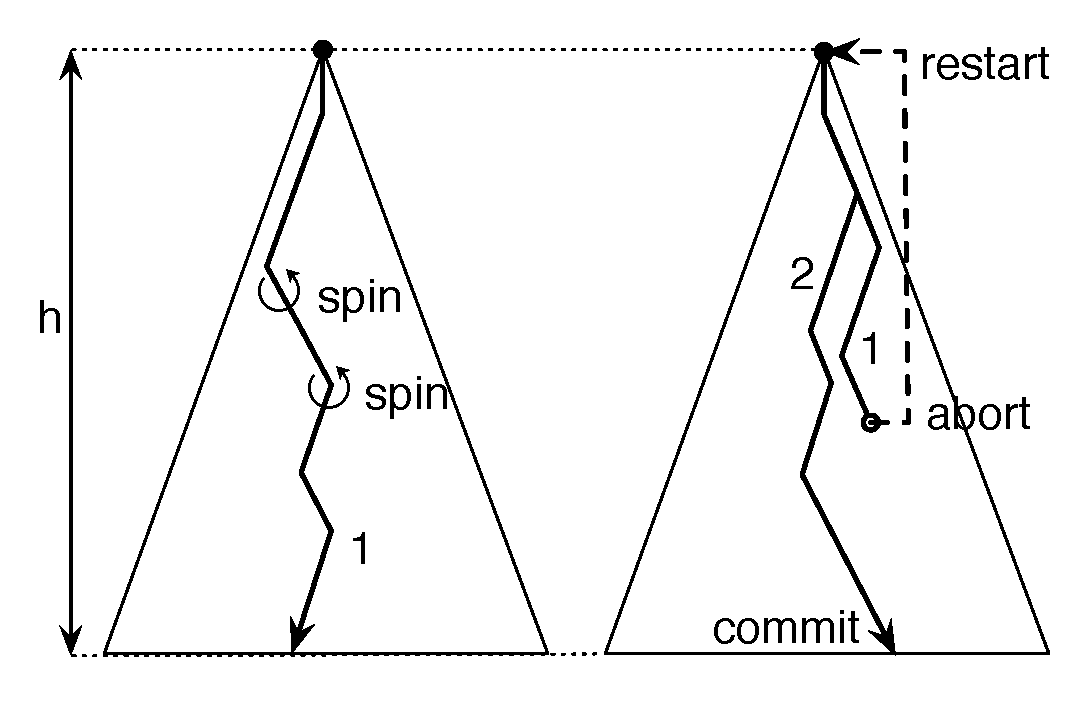
\includegraphics[scale=0.4]{Tree/fig/complexity}
% 	\caption{A balanced search tree whose complexity, in terms of the amount of accessed elements, is {\bf (left)} proportional to $h$ 
% 	in a pessimistic execution and {\bf (right)} proportional to the number of restarts in an optimistic execution\label{fig:complexity}}
% 	\end{center}
% \end{figure}
% 
% To illustrate the difference between optimistic and pessimistic 
% synchronizations consider the example of 
% % example
% Figure~\ref{fig:complexity} depicting their step complexity when
% traversing a tree of height $h$ from its root to a leaf node. On the left, 
% steps are executed pessimistically, potentially spinning before being able to acquire 
% a lock, on the path converging towards the leaf node. On the right, 
% steps are executed optimistically and some of them
% may abort and restart, depending on concurrent thread steps. The pessimistic 
% execution of each thread is guaranteed to execute $O(h)$ steps, yet the optimistic one 
% may need to execute $\Omega(hr)$ steps, where $r$ is the number of restarts. 
% Note that $r$ depends 
% on the probability of conflicts with concurrent transactions that depends, in turn, 
% on the transaction length and $h$.


When considering implementing a tree using TM it is clear that, although a transaction must be aborted before violating 
the abstraction implemented by this tree
(e.g., inserting $k$ successfully in a set where $k$ has already been inserted by a concurrent transaction),
it is unclear whether a transaction must be aborted due to
slightly unbalancing the tree implementation in order to strictly preserve the balance invariant.
Following this assumption we introduce a \emph{speculation-friendly} tree as a tree that transiently breaks its
balance structural invariant without hampering the abstraction consistency in order to speed up transaction-based accesses. 
Here are our contributions.

\begin{itemize}
\item We propose a speculation-friendly binary search tree data structure
implementing an associative array and set abstractions.
In this implementation we decouple the operations that modify the abstraction (we call these \emph{abstract transactions}) from operations
that modify the tree structure itself but not the abstraction (we call these \emph{structural transactions}).
An abstract transaction either inserts or deletes an element from the abstraction and 
in certain cases the insertion might also modify the tree structure.
Structural transactions have two main tasks:
(1) Certain structural transactions are given the task to balance the tree 
by executing a distributed rotation mechanism: each of these transactions executes a local rotation involving
only a constant number of neighboring nodes. 
(2) Some other structural transactions unlink and free nodes that have been logically deleted 
by previously committed abstract transactions.

\item We prove the correctness (i.e., linearizability) of our tree and we compare its performance against existing transaction-based versions of an AVL tree and a red-black tree,
widely used to evaluate transactions~\cite{DSS06,HLMS03,CCKO08,HK08,FFR08,YNW+08,DFGG11}.
The speculation-friendly tree improves by up to $1.6\times$ the performance of the AVL tree on the micro-benchmark and 
by up to $3.5\times$ the performance of the built-in red-black tree on a travel reservation application, already well-engineered for transactions.
Finally, our speculation-friendly tree performs similarly to a non-rotating tree but remains robust in face of non-uniform workloads.

\item We illustrate (i)~the portability of our speculation-friendly tree by evaluating it on two different Transactional Memories (TMs), TinySTM~\cite{FFR08} 
and $\mathcal{E}$-STM~\cite{FGG09} and with different configuration settings, hence outlining that our performance benefit is independent 
from the transactional algorithm it uses; and (ii)~how it can be reused by composing 
straightforwardly the $\lit{remove}$ and $\lit{insert}$ into a new $\lit{move}$ operation.
In addition, we compare the benefit of relaxing data structures into speculation-friendly ones against the benefit of only relaxing transactions,
by evaluating elastic transactions.
It shows that, for a particular data structure, refactoring its algorithm is preferable to refactoring the underlying transaction algorithm.
\end{itemize}

% The chapter is organized as follows. In Section~\ref{sec:pb} we describe the problem related
% to the use of transactions in existing balanced trees. In Section~\ref{sec:tf} we present our 
% speculation-friendly binary search tree. In Section~\ref{sec:expe} we evaluate our tree
% experimentally and illustrate its portability and reusability.
% In Section~\ref{sec:rw} we describe the related work and 
% Section~\ref{sec:conclusion} concludes.





\section{Conclusion}
% Given that this definition gives no details on the complex interactions of transactions in
% the system, instead of trying to expand this definition with further details,
This thesis looks at possible solutions to deal with the difficulties that come up when
a programmer uses transactional memory, taking ease of use as the primary concern.
Even though precise definitions of semantics and properties are used as solutions
for the specific problems the goal is that they relate directly with the high level interface they define.
Therefore, a programmer who
understands the high level definition should find the specific details of the low level definitions as a
natural extension.

The grand goal is that someday a programmer can write an efficient concurrent program
with nearly as much ease as he would write a sequential one.
While this goal is far from fully achieved here,
this thesis makes important steps in this direction, while suggesting ways to move forward further.






